\documentclass[a4paper,10pt,titlepage]{article}

\usepackage[utf8]{inputenc}
\usepackage[ngerman]{babel}
\usepackage{graphicx}
\usepackage{a4wide}
\usepackage{url}
\usepackage{booktabs}
\usepackage{float}

\usepackage[pdfborder={0 0 0}]{hyperref}

\graphicspath{{./grafiken/}}

\author{ToureNPlaner Team}
\title{Spezifikation ToureNPlaner\\ Stupro 2011/2012}

\newcommand{\shortcut}[1]
{\texttt{#1}}

\newcommand{\usecase}[8]
{\subsection{#1}
\begin{tabular}{|p{0.2\textwidth}|p{0.7\textwidth}|}
\hline
  Akteur & #2\\\hline
  Ziel & #3\\\hline
  Vorbedingung & #4\\\hline
  Normalablauf & #7\\\hline
  Nachbedingung & #5\\\hline
  Sonderfall & #8\\\hline
  Nachbedingung im Sonderfall& #6\\\hline
 \end{tabular}
}

\newcommand{\begriff}[7]
{\subsection{#1}
\begin{tabular}{|p{0.2\textwidth}|p{0.7\textwidth}|}
\hline
  Bedeutung & #2\\\hline
  Abgrenzung & #3\\\hline
  Gültigkeit & #4\\\hline
  Bezeichnung & #5\\\hline
  Unklarheiten & #6\\\hline
  Querverweise & #7\\\hline
 \end{tabular}}

\newcommand{\doaction}[1]
{Der Benutzer führt die Aktion „\nameref{#1}“ (\ref{#1}) aus.}

\begin{document}

\pagenumbering{alph}
\maketitle
\pagenumbering{roman}
\setcounter{page}{1}
\tableofcontents
\clearpage
\pagenumbering{arabic}
\setcounter{page}{1}

\section{Einleitung}
\subsection{Zweck der Spezifikation}
Die Spezifikation beschreibt die Anforderungen und Funktionalitäten von Tourenplaner. Sie ist die Grundlage für alle folgenden Dokumente; insbesondere muss sie ständig mit dem Entwurf verglichen und bei Bedarf angepasst werden.

Bei der Erstellung der Spezifikation wurde bewusst auf die Festlegung von Implementierungsdetails verzichtet, um gewisse Freiheiten in der Umsetzung der Anforderungen zu erhalten.

\subsection{Leserkreis}
Der Leserkreis dieses Dokuments besteht aus folgenden Personengruppen:
\begin{itemize}
\item Die Entwickler
\item Die Beteiligten des Spezifikationsreviews
\item Der Kunde
\item Die Betreuer des Studienprojekts
\end{itemize}

\subsection{Einsatzbereich und Ziele}

In diesem Project sollen die Clients für das ToureNPlaner-Projekt realisiert werden.
Diese dienen der einfachen Nutzung der Funktionalitäten, die der ToureNPlaner-Server zur Verfügung steht.
Dazu soll es möglich sein, einfach Strecken und Touren zu definieren und vom Server berechnen zu lassen.

\noindent Das Ziel ist es, zu kommerziellen bzw. marktführenden Lösungen konkurrenzfähige Clients zu erstellen.

\subsection{Fachbegriffe und Abkürzungen}

Alle in dieser Spezifikation verwendeten Fachbegriffe werden im sich im Anhang befindlichen Begriffslexikon erläutert.

\subsection{Aufbau dieses Dokuments}

Neben einer allgemeinen Beschreibung des Systems sollen die Anforderungen an die Funktionen des Systems und die geforderten Qualitäten hinsichtlich der Software dokumentiert werden. 
Im Anschluß hierzu wird auf die Benutzeroberfläche und im nächsten Schritt auf die Anwendungsfälle des Systems näher eingegangen. 
Das Dokument endet schließlich mit einem angehängten Begriffslexikon.

\section{Nichtfunktionale Anforderungen}
\subsection{Mengengerüst}
\label{Mengengeruest}
Die mindest Punktanzahl um einen sinnvollen Weg zu berechnen beträgt 2.
Nach obenhin soll ToureNPlaner mit bis zu 100 Punkten zurecht kommen.\\
Der Client wird immer nur von einem Benutzer gleichzeitig verwendet.

\subsection{Entwurfseinschränkungen}
\subsubsection{Systemumgebung}
Der Webclient wir auf der aktuellen Version von Firefox - Version 5 - und Chromium - Version 13 - lauffähig sein.\\
Für Android setzten wir Version 2.1 oder neuer voraus.

\subsubsection{Layout und Gestaltung}
Die Oberfläche wir beim Webclient mit Hilfe von HTML 5 und CSS 3, die des Androidclient mit XML und den Android Developer Tools umgesetzt.

\subsubsection{Datenhaltung}
\label{datenhaltung}
Im Webclient werden die benötigten Daten in Cookies abgelegt.\\
Der Androidclient benutz hierzu eine Konfigurations-API.

\subsection{Robustheit}
Der Webclient verfügt über keine besondere Robustheit.\\
Auf Android können Daten wiederhergestellt werden.

\subsection{Portabilität}
Der Webclient ist gut auf andere Browser adaptierbar.\\
Android ist wegen des ADTs nur auf Android-Geräten lauffähig.

\subsection{Erweiterbarkeit}
Alle Informationen über Algorithem kommt vom Server, deshalb können einfach neue Algorithem hinzugefügt werden.
Daher werden nur Algorithem unterstützt, welche mit Pfaden auf einem Graphen arbeiten.

\subsection{Distributionsform und Installation}
Zur Installation müssen die Daten für die Webclienten auf den Webserver kopiert werden.\\
Für den Androidclient werden Android Packages (APKs) verfügbar sein.

\subsection{Sprachunterstützung}
Beide Client haben dieselbe Übersetztungsdateien als Grundlange, somit soll Konsitenz gewährleistet werden.
Die Übersetzungen werden mit Hilfe von GNU gettext implementiert.

\clearpage
\section{Funktionale Anforderungen}
\subsection{Anmeldung und Registrierung}
Kostenpflichtige als auch kostenlose Berechnungen sollen nur nach Anmeldung am Client möglich sein.
Besitzt ein User noch keinen Account, so kann er diesen erhalten, nachdem er eine Registrierung am WebClient durchgeführt hat.

\subsection{Angaben zur Berechnung}
Am Client soll der User zunächst einen Algorithmus auswählen, mit dem er eine Berechnung durchführen möchte.
Anschließend soll er mithilfe der Karte folgende Operationen durchführen können, 
bevor er seine Berechnung an den Server abschickt:
\begin{itemize}
 \item Start- und Zielpunkt setzen
 \item ggfs. weitere Punkte hinzufügen
 \item bereits gesetzte Punkte editieren
 \item bereits gesetzte Punkte löschen.
\end{itemize}
Hat der User seine Angaben zum Algorithmus getätigt, so kann er diese letzendlich zum Server abschicken.

\subsection{Betrachten des Ergebnis}
Nachdem das Ergebnis vom Server zurückgesendet wurde, soll dieses in Form einer Route auf der Karte angezeigt werden.
Dem User sollen dabei folgende Funktionen zur Verfügung stehen:
\begin{itemize}
 \item hinein- und hinauszoomen
 \item auf der Karte navigieren (Karte mit der Maus verschieben)
\end{itemize}

\subsection{Benutzerverwaltung}
Der User soll seine Benutzerdaten anzeigen und bearbeiten können.

\subsection{Billing}
Der User soll über den WebClient Zugriff auf seine Billing-Informationen haben.


\subsection{Administration}
Der Administrator soll auf eine Übersicht aller Benutzer zugreifen können, auf der folgende Funktionalitäten verfügbar sind:
\begin{itemize}
 \item Benutzer anlegen
 \item Benutzer bearbeiten
 \item Benutzer löschen
\end{itemize}

Zudem soll er eine Übersicht aller getätigten Requests erhalten.

\clearpage
\section{Benutzeroberfläche}
\subsection{Web-Client}
\subsubsection{Überblick}
Die Benutzeroberfläche des Web-Clients wird folgende Funktionen ermöglichen
\begin{itemize}
\item Auswahl eines Servers
\item Anmelden mit Benutzernamen und Kennwort
\item ’Passwort vergessen?’ Funktion
\item Benutzerverwaltung
\item Auswahl des gewünschten Algorithmus
\item Auswahl der Billing-Anzeige 
\item Kartenansicht
\item Marker auf der Karte anlegen
\item Marker Eigenschaften zuweisen
\item Route berechnen
\item Route auf der Kartenansicht anzeigen
\end{itemize}
\subsubsection{Darstellung des Web-Clients}
Folgende Abbildungen sollen als Vorlage zur genauen Realisierung dienen.
%TODO insert screenshots
\subsubsection{Kartenansicht}
Hier kann der Benutzer auf der eingeblendeten Kartenansicht folgende Operationen durchführen.
\begin {itemize}
\item kurzer Linksklick erstellt einen Marker an dieser Position 
\item kurzer Rechtsklick noch nicht definiert
\item Drücken auf einen Marker ermöglicht das Verändern der Eigenschaften dieses Markers
\item gedrückter Linksklick ziehen auf der Karte ändert den Fokus der Kartenansicht
\item die Benutzund des Mausscrollrades ermöglicht die Änderung des momentanen Zoomfaktors auf der Kartenansicht 
\end {itemize}
%TODO insert screenshots
Nachdem die Route berechnet wurde, kann das Ergebnis anhand eines angezeigten Pfades auf der Karte nachvollzogen werden.

\newpage
\subsection{Android-Client}
\subsubsection{Überblick}
Die Benutzeroberfläche des Android-Clients wird folgende Funktionen ermöglichen
\begin{itemize}
\item Auswahl eines Servers
\item Anmelden mit Benutzernamen und Kennwort
\item 'Passwort vergessen?' Funktion
\item Auswahl des gewünschten Algorithmus
\item Auswahl der Billing-Anzeige 
\item Kartenansicht
\item Marker auf der Karte anlegen
\item Marker Eigenschaften zuweisen
\item Route berechnen
\item Route auf der Kartenansicht anzeigen
\end{itemize}
\subsubsection{Darstellung des Android-Clients}
Es folgen nun Layouts aller Aktivities, die als Vorlage zur genauen Realisierung dienen sollen.

\subsubsection{Auswahl des Servers}
Hier kann der Benutzer einen gewünschten Server auswählen.
\begin {center}
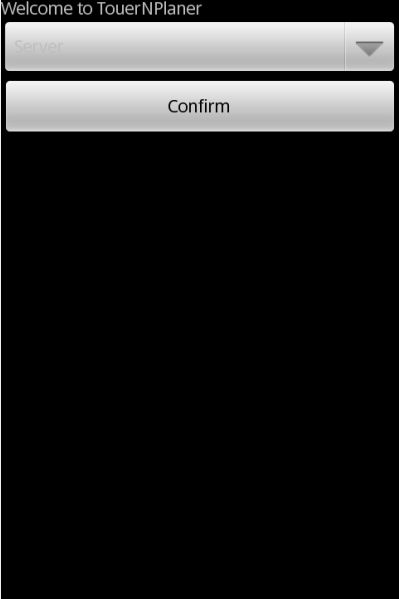
\includegraphics[scale=0.40]{media/android/server.jpg}
\end {center}

\subsection{Anmeldeinformationen}
Hier kann der Benutzer seine Anmeldeinformationen eingeben und sich mit dem Server verbinden.
\begin {center}
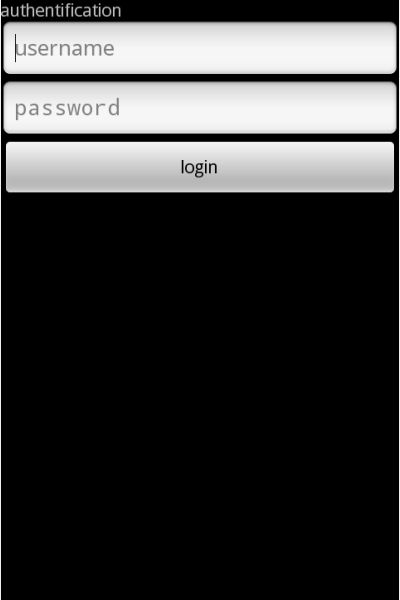
\includegraphics[scale=0.35]{media/android/login.jpg}
\end {center}

\subsection{Algorithmus auswählen}
Hier kann der Benutzer den von ihm gewünschten Algorithmus auswählen.
\begin {center}
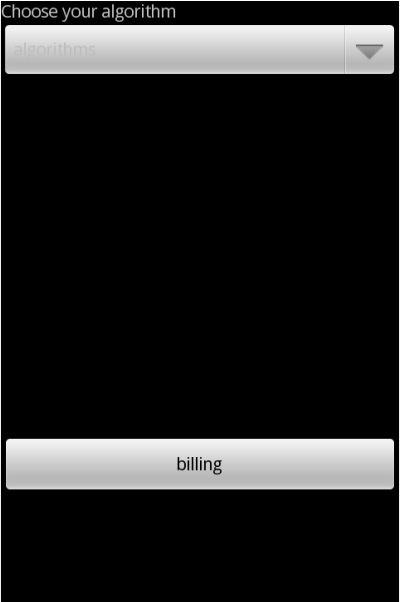
\includegraphics[scale=0.47]{media/android/algorithms.jpg}
\end {center}

\newpage
\subsection{Kartenansicht}
Hier kann der Benutzer auf der eingeblendeten Kartenansicht folgende Operationen durchführen.
\begin {itemize}
\item kurzes Drücken ist noch nicht definiert
\item langes Drücken erstellt einen Marker an dieser Position
\item Drücken auf einen Marker ermöglicht das Verändern der Eigenschaften dieses Markers
\item Ziehen auf der Karte ändert den Fokus der Kartenansicht
\item Klicken auf einen der Zoom-Schaltflächen ermöglicht die Änderung des momentanen Zoomfaktors auf der Kartenansicht 
\end {itemize}
Nachdem die Route berechnet wurde, kann das Ergebnis anhand eines angezeigten Pfades auf der Karte nachvollzogen werden.

\begin {center}
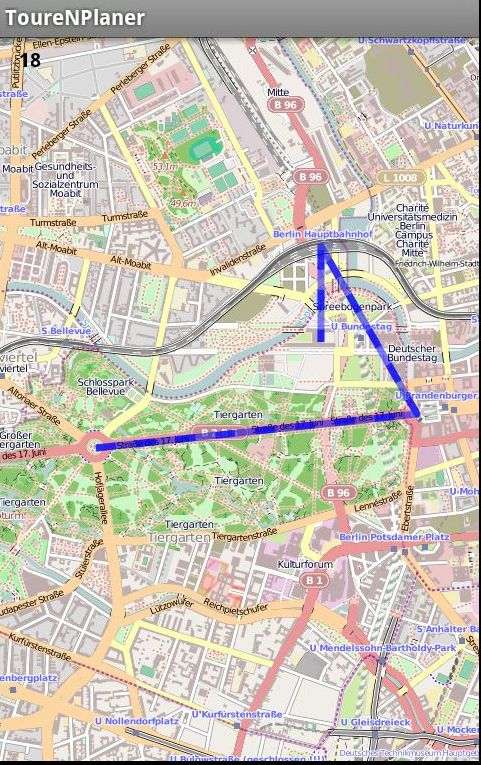
\includegraphics[scale=0.4]{media/android/map.jpg}
\end {center}
\newpage



\clearpage
\section{Anwendungsfälle (Use-Cases)}
\begin{figure}[H]
  \centering
  %TODO
  %\includegraphics[width=\linewidth]{usecases.png}
  \caption{Usecase-Diagramm}
\end{figure}

%\usecase{Name}{Akteur}{Ziel}{Vorbedingung}{Nachbedingung}{Nachbedingung im Sonderfall}{Normalablauf}{Sonderfall}
\subsection*{Benutzeroberflächenfunktionen}
\usecase{Algorithmus auswählen}{Benutzer}{Algorithmus auswählen}{Der Benutzer ist am Server angemeldet}{Der Benutzer hat einen Algorithmus ausgewählt}{Der Benutzer bekommt eine Fehlermeldung}{1. Der Benutzer wählt seinen Algorithmus \newline 2. Benutzer bestätigt seine Eingabe}{Die Verbindung zum Server wurde unterbrochen}

\usecase{Marker hinzufügen}{Benutzer}{Einen Marker auf der Karten hinzufügen}{Die Karte wird angezeigt}{Ein Marker wurde an die gewünschte Stelle plaziert}{Der Marker konnte nicht angelegt werden}{1. Der Benutzer wählt einen gewünschten Punkt auf der Karte \newline 2. Der Benutzer erstellt dort einen Marker}{ungültiger Bereich}

\usecase{Marker editieren}{Benutzer}{Einen vorhandenen Marker editieren}{Ein Marker muss existieren}{Der Marker wurde editiert}{Der Marker wurde auf seine vorherigen Werte zurückgesetzt}{1. Der Benutzer wählt einen Marker aus \newline 2. Der Benutzer ändert die gewünschten Werte des Markers \newline 3. Der Benutzer bestätigt seine Eingaben}{ungültige Eingaben}

\usecase{Marker löschen}{Benutzer}{Einen vorhandenen Marker löschen}{Ein Marker muss vorhanden sein}{Der Marker wurde gelöscht}{keine}{1. Der Benutzer wählt einen Marker aus \newline 2. Der Benutzer bestätigt das Löschen}{keine}

\usecase{Start/Zielpunkt setzen}{Benutzer}{Einen Marker als Ziel/Startpunkt setzen}{Ein Marker muss vorhanden sein}{Ein Marker ist Start/Zielpunkt}{keine}{1. Der Benutzer wählt einen Marker aus \newline 2. Der Benutzer setzt ihn als Start/Zielpunkt}{keine}

\usecase{Route berechnen}{Benutzer}{Eine Route berechnen}{Es müssen Marker auf der Karte plaziert worden sein}{Eine Route wurde berechnet}{Es wurde eine Fehlermeldung geworfen}{1. Der Benutzer bestätigt seine Eingaben \newline 2. Der Benutzer berechnet seine Route}{Benötigte angaben für die Berechnung fehlen}

\usecase{Route anzeigen}{Benutzer}{Die Route nachverfolgen können}{Eine Route muss berechnet worden sein}{Es wurde eine Route auf die Kartenansicht gezeichnet}{Es wurde eine Fehlermeldung ausgegeben}{1. Der Benutzer wählt Route anzeigen aus}{Bei der Berechnung der Route traten Fehler auf}

\subsection*{Benutzerverwaltungsfunktionen}
\usecase{Benutzer registrieren}
{Benutzer}{Der Benutzer will sich ein Benutzerkonto anlegen.}{Keine}{Das Konto wurde erfolgreich im System angelegt.}{Der Benutzer sieht eine Fehlermeldung.}{
\begin{enumerate}
\item Der Benutzer navigiert zum Registrierungsformular.
\item Der Benutzer gibt seine Daten ein.
\item Der Benutzer bestätigt seine Angaben.
\end{enumerate}
}{Es gab einen Fehler beim Erstellen des Kontos.}

\usecase{Anmelden}
{Benutzer}{Der Benutzer will sich am System anmelden.}{Keine}{Der Benutzer ist am System angemeldet.}{Der Benutzer sieht eine Fehlermeldung.}{
\begin{enumerate}
\item (optional) Der Benutzer wählt den Server aus.
\item Der Benutzer gibt seine Anmeldedaten ein.
\item Der Benutzer bestätigt seine Angaben.
\end{enumerate}
}{Die Anmeldedaten sind falsch.}

\usecase{Benutzerdaten anzeigen}
{Benutzer}{Der Benutzer will seine Daten einsehen.}{Der Benutzer hat sich eingeloggt.}{Der Benutzer sieht seine Daten.}{Der Benutzer sieht eine Fehlermeldung.}{
\begin{enumerate}
\item Der Benutzer navigiert zur Benutzerdatenansicht.
\item Der Benutzer sieht seine Daten.
\end{enumerate}
}{Es gibt einen Fehler.}

\usecase{Benutzerdaten bearbeiten}
{Benutzer}{Der Benutzer will seine Daten bearbeiten.}{Der Benutzer hat sich eingeloggt.}{Die Daten des Benutzers sind geändert.}{Der Benutzer sieht eine Fehlermeldung.}{
\begin{enumerate}
\item Der Benutzer navigiert zur Benutzerdatenansicht.
\item Der Benutzer ändert seine Daten.
\item Der Benutzer bestätigt seine Angaben.
\end{enumerate}
}{Es gibt einen Fehler.}

\usecase{Abrechnung anzeigen}
{Benutzer}{Der Benutzer will seine Abrechnung sehen.}{Der Benutzer hat sich eingeloggt.}{Der Benutzer sieht seine Abrechnung.}{Der Benutzer sieht eine Fehlermeldung.}{
\begin{enumerate}
\item Der Benutzer navigiert zur Abrechnungsansicht.
\item Der Benutzer sieht seine Abrechnung.
\end{enumerate}
}{Es gibt einen Fehler.}

\usecase{Alte Abfrage anzeigen}
{Benutzer}{Der Benutzer will eine alte Route sehen.}{Der Benutzer hat sich eingeloggt.}{Der Benutzer sieht seine alte Route.}{Der Benutzer sieht eine Fehlermeldung.}{
\begin{enumerate}
\item Der Benutzer navigiert zur Abrechnungsansicht.
\item Der Benutzer wählt eine alte Abfrage aus.
\item Der Benutzer sieht seine alte Abfrage.
\end{enumerate}
}{Es gibt einen Fehler.}

\clearpage
\appendix
\section{Anhang}

\subsection{Begriffslexikon}

%\begriff{Begriff}{Bedeutung}{Abgrenzung}{Gültigkeit}{Bezeichnung}{Unklarheiten}{Querverweise}

\clearpage
\subsection{Versionshistorie}

	\subsubsection*{Version 0.1 (03.08.2011)}
	\begin{itemize}
		\item Erste veröffentlichte Version
	\end{itemize}

	\subsubsection*{Version 0.2 (09.08.2011)}
	\begin{itemize}
		\item Nichtfunktionale Anforderungen hinzugefügt
	\end{itemize}

\end{document}
